\chapter{Referencial Teórico}

Este capítulo apresenta os conceitos fundamentais que embasam a pesquisa, organizados em quatro seções principais. Inicialmente, são abordados os conceitos gerais de bancos de dados e o modelo relacional, estabelecendo a base teórica necessária. Em seguida, são discutidos os bancos de dados distribuídos, essenciais para compreender a escalabilidade em ambientes modernos. Na sequência, são explorados os bancos de dados de séries temporais (TSDBs), foco central deste trabalho. Por fim, são apresentados os métodos de avaliação de desempenho através de benchmarks, fundamentais para a análise comparativa proposta.

\section{Banco de Dados}

Segundo \citeonline{Ramakrishnan2003}, um banco de dados pode ser definido por uma coleção de dados, tipicamente descrevendo as atividades de uma ou mais organizações relacionadas. Esta definição abrange desde informações sobre entidades, como estudantes e cursos em uma universidade, até os relacionamentos entre essas entidades, como a matrícula de alunos em disciplinas específicas. Em \citeonline{Silberschatz2020} argumenta-se ainda que o principal objetivo de um banco de dados deve ser fornecer uma maneira de recuperar informações que seja tanto conveniente quanto eficiente.

O gerenciamento desses dados é realizado por um Sistema de Gerenciamento de Banco de Dados (SGBD), que é um software projetado para auxiliar na manutenção e utilização de grandes coleções de dados \cite{Ramakrishnan2003}. Os autores destacam que a necessidade por tais sistemas tem crescido rapidamente, sendo a alternativa ao uso de um SGBD a adoção de abordagens ad-hoc que não são transferíveis de uma aplicação para outra, como armazenar os dados em arquivos e escrever código específico para gerenciá-los.

A importância dos bancos de dados na era da informação é ressaltada pelos autores quando afirmam que o sucesso de uma organização depende cada vez mais de sua capacidade de adquirir dados precisos e oportunos sobre suas operações, gerenciar esses dados efetivamente e usá-los para analisar e guiar suas atividades \citeonline{Ramakrishnan2003}. Esta afirmação reflete o papel central que os bancos de dados assumiram nas organizações modernas, onde a informação é reconhecida como um ativo estratégico.

\citeonline{Ramakrishnan2003} apresentam diversas vantagens no uso de um SGBD em comparação com sistemas de arquivos tradicionais. Entre elas destacam-se a independência de dados, que isola os programas aplicativos dos detalhes de representação e armazenamento; o acesso eficiente aos dados, possibilitado por técnicas sofisticadas de armazenamento e recuperação; a integridade e segurança dos dados, permitindo que o SGBD restrinja acessos não autorizados; e o suporte a acesso concorrente e recuperação após falhas.

O modelo relacional, proposto por Codd em 1970, revolucionou a área de bancos de dados e substituiu em grande parte os modelos hierárquico e de rede que o precederam. Segundo os autores, este modelo é simples e elegante, onde um banco de dados é visto como uma coleção de relações (tabelas com linhas e colunas), sendo que esta representação tabular permite até mesmo usuários iniciantes compreenderem facilmente os conteúdos armazenados \citeonline{Ramakrishnan2003}.

A estruturação dos dados no modelo relacional é baseada em relações, que consistem em um esquema da relação e uma instância da relação \citeonline{Ramakrishnan2003}. O esquema especifica o nome da relação, o nome de cada campo (ou coluna) e o domínio de cada campo, enquanto a instância é um conjunto de tuplas (registros) onde cada tupla possui o mesmo número de campos que o esquema da relação. Os autores enfatizam que cada relação é definida para ser um conjunto de tuplas únicas, o que garante a não duplicação de registros.

Para garantir a qualidade e consistência dos dados armazenados, os bancos de dados utilizam restrições de integridade (ICs), que são condições especificadas no esquema do banco de dados e que restringem os dados que podem ser armazenados em uma instância do banco de dados \citeonline{Ramakrishnan2003}. Quando uma instância de banco de dados satisfaz todas as restrições de integridade especificadas no esquema do banco de dados, dizemos que é uma instância legal, e o SGBD deve garantir que apenas instâncias legais sejam armazenadas.

Mesmo assim, é importante que o banco de dados ofereça para os usuários uma visão abstrata dos dados, ou seja, ocultando certos detalhes de como os dados são armazenados ou mantidos, argumenta \citeonline{Silberschatz2020}. Deve servir como abstração para resolução de problemas reais de maneira eficiente e prática.

Entre os principais tipos de restrições de integridade destacam-se as restrições de chave, que afirmam que um subconjunto mínimo dos campos de uma relação é um identificador único para uma tupla, e as restrições de chave estrangeira, que ocorrem quando a informação em uma relação está ligada à informação em outra relação. Estas restrições são fundamentais para manter a consistência dos dados quando múltiplas tabelas estão relacionadas.

A linguagem SQL tornou-se o padrão para interação com bancos de dados relacionais. Como observam \citeonline{Ramakrishnan2003}, SQL é a linguagem comercial mais popular para SGBDs relacionais. A linguagem permite não apenas a definição da estrutura dos dados, mas também sua manipulação e consulta, sendo que uma consulta ao banco de dados relacional é definida como uma pergunta sobre os dados, cuja resposta consiste em uma nova relação contendo o resultado.

O projeto de um banco de dados relacional frequentemente começa com um diagrama Entidade-Relacionamento (ER), que é conveniente para representar um projeto inicial de alto nível. Os autores descrevem um método padrão para traduzir um diagrama ER em um esquema de banco de dados relacional que se aproxima do projeto ER original, embora com algumas limitações na representação de certas restrições usando apenas SQL-92.

Em resumo, os bancos de dados representam a principal tecnologia para armazenamento e gerenciamento de informações nas organizações modernas, oferecendo vantagens significativas em termos de eficiência, segurança e consistência dos dados quando comparados a abordagens alternativas de armazenamento. O modelo relacional, com sua simplicidade e poder de expressão, consolidou-se como o paradigma dominante na área, sendo implementado pela maioria dos sistemas comerciais atuais.

\section{Bancos de Dados Distribuídos}

Os bancos de dados distribuídos (BDDs) representam a convergência entre duas tecnologias aparentemente opostas: sistemas de banco de dados e redes de computadores \citeonline{Ozsu2011}. Enquanto os sistemas de banco de dados tradicionais promovem a centralização dos dados para garantir controle e integridade, as redes de computadores incentivam a distribuição e descentralização. A tecnologia de BDDs sintetiza esses conceitos, demonstrando que a integração dos dados não necessariamente implica na sua centralização física.

Para \citeonline{Silberschatz2020}, de maneira similar, um sistema de banco de dados distribuído é composto por várias instâncias com bancos locais, capazes de processar transações locais. Também podem executar transações globais, que acessam dados em múltiplos sites, exigindo comunicação entre eles.

Um \textit{banco de dados distribuído} é definido como uma coleção de múltiplos bancos de dados logicamente inter-relacionados, distribuídos por uma rede de computadores \citeonline{Ozsu2011}. O sistema de gerenciamento de banco de dados distribuído (SGBDD) é o software que permite o gerenciamento desse banco de dados distribuído, tornando a distribuição transparente para os usuários. É importante destacar que um BDD não é simplesmente um conjunto de arquivos armazenados em diferentes nós de uma rede, mas sim um sistema estruturado com esquema definido e acesso através de uma interface comum.

A arquitetura de um SGBDD pode ser organizada de diferentes formas, sendo as principais: sistemas \textit{cliente/servidor}, sistemas \textit{peer-to-peer} (ponto-a-ponto) e sistemas \textit{multibanco de dados} \citeonline{Ozsu2011}. Nos sistemas cliente/servidor, as funções são divididas entre clientes (que gerenciam a interface com o usuário) e servidores (responsáveis pelo gerenciamento dos dados). Já nos sistemas peer-to-peer, todas as máquinas possuem funcionalidade completa de SGBD e podem se comunicar diretamente para executar consultas e transações. Os sistemas multibanco de dados lidam com a integração de bancos de dados heterogêneos e autônomos.

Uma das principais promessas dos BDDs é o gerenciamento transparente de dados distribuídos e replicados. Essa transparência se manifesta em vários níveis: independência de dados (imunidade das aplicações a mudanças na estrutura lógica ou física dos dados), transparência de rede (proteção do usuário contra detalhes operacionais da rede), transparência de replicação (ocultação da existência de cópias múltiplas dos dados) e transparência de fragmentação (divisão das relações em fragmentos tratados como objetos independentes). Como destacam \citeonline{Ozsu2011}, o objetivo mais importante da tecnologia de banco de dados é a integração, não a centralização.

\citeonline{Silberschatz2020} afirma que bancos de dados distribuídos podem ser homogêneos ou heterogêneos, que são, respectivamente, sistemas de banco de dados em que os esquemas ou código são comuns entre as instâncias ou que diferem entre cada instância.

Os BDDs oferecem maior confiabilidade através do suporte a transações distribuídas. Uma transação é definida como uma unidade básica de computação confiável e consistente, consistindo em uma sequência de operações de banco de dados executadas como uma ação atômica. Em um ambiente distribuído, as transações podem ser executadas em vários sites, acessando bancos de dados locais. Com suporte completo a transações distribuídas, os usuários podem acessar uma única imagem lógica do banco de dados, confiando no SGBDD para garantir que suas requisições serão executadas corretamente, independentemente de falhas no sistema.

O desempenho em BDDs pode ser melhorado através da localização dos dados (armazenamento próximo aos pontos de uso) e do aproveitamento do paralelismo inerente dos sistemas distribuídos. A localização reduz a contenção por serviços de CPU e E/S, enquanto o paralelismo pode ser explorado tanto entre consultas (\textit{inter-query}) quanto dentro de uma única consulta (\textit{intra-query}) \citeonline{Ozsu2011}. No entanto, como alertam \citeonline{Ozsu2011}, a mistura de operações de leitura e atualização requer a implementação de elaborados protocolos de controle de concorrência.

Entre os principais desafios dos BDDs estão a replicação de dados, o tratamento de falhas e a sincronização de transações em múltiplos sites. \citeonline{Silberschatz2020} aponta que a detecção de impasse em sistemas distribuídos exige cooperação entre sites, pois podem ocorrer impasses globais mesmo sem impasses locais.

A replicação introduz complexidade na manutenção da consistência entre as cópias dos dados. As falhas de sites ou enlaces de comunicação exigem mecanismos para garantir que os efeitos das atualizações sejam refletidos em todos os locais assim que o sistema se recuperar. Além disso, como cada site não tem informação instantânea sobre as ações que estão sendo executadas nos outros sites, a sincronização de transações se torna significativamente mais complexa do que em sistemas centralizados.

Os problemas de projeto em SGBDDs incluem: projeto do banco de dados distribuído (fragmentação e distribuição ótima dos dados), gerenciamento de diretórios distribuídos, processamento de consultas distribuídas, controle de concorrência distribuído, gerenciamento de deadlock distribuído, confiabilidade do SGBDD e protocolos de replicação . Como destacam \citeonline{Ozsu2011}, esses problemas não são isolados, mas sim inter-relacionados, onde a solução de um afeta os outros.

A arquitetura de referência para SGBDDs peer-to-peer, conforme apresentada por \citeonline{Ozsu2011}, inclui três níveis de esquema: esquema conceitual global (visão lógica de todos os dados no sistema), esquema conceitual local (organização lógica dos dados em cada site) e esquema interno local (organização física em cada site). Essa arquitetura é implementada através de dois componentes principais: o \textit{processador do usuário} (que lida com a interface do usuário, controle semântico, otimização de consultas e monitoramento de execução) e o \textit{processador de dados} (responsável pelo processamento local de consultas, gerenciamento de recuperação e suporte à execução).

Bancos de dados distribuídos representam uma evolução natural dos sistemas de banco de dados em um mundo cada vez mais conectado, oferecendo benefícios significativos em termos de transparência, confiabilidade e desempenho, mas também introduzindo complexidades adicionais no gerenciamento da distribuição dos dados e do processamento das transações.

\subsection{Bancos de Dados de Séries Temporais}

Os bancos de dados de séries temporais (TSDB - \textit{Time Series Databases}) representam uma categoria especializada de sistemas de armazenamento projetados para lidar com dados que são registrados como uma sequência de valores, cada um associado a um momento temporal específico. Segundo \citeonline{Ozsu2011}, uma série temporal é um conjunto de valores de atributos ao longo de um período de tempo. Essa característica fundamental diferencia os TSDBs dos bancos de dados tradicionais, pois eles são otimizados para consultas baseadas em intervalos de tempo, oferecendo desempenho superior para esse padrão de acesso.

Registros meteorológicos, indicadores econômicos e métricas de evolução da saúde do paciente — todos são dados de séries temporais. Dados de séries temporais também podem incluir métricas de servidor, monitoramento de desempenho de aplicativos, dados de rede, dados de sensores, eventos, cliques e muitos outros tipos de dados analíticos. \citeonline{InfluxDataTimeSeries}.

\begin{figure}[h]
    \centering
    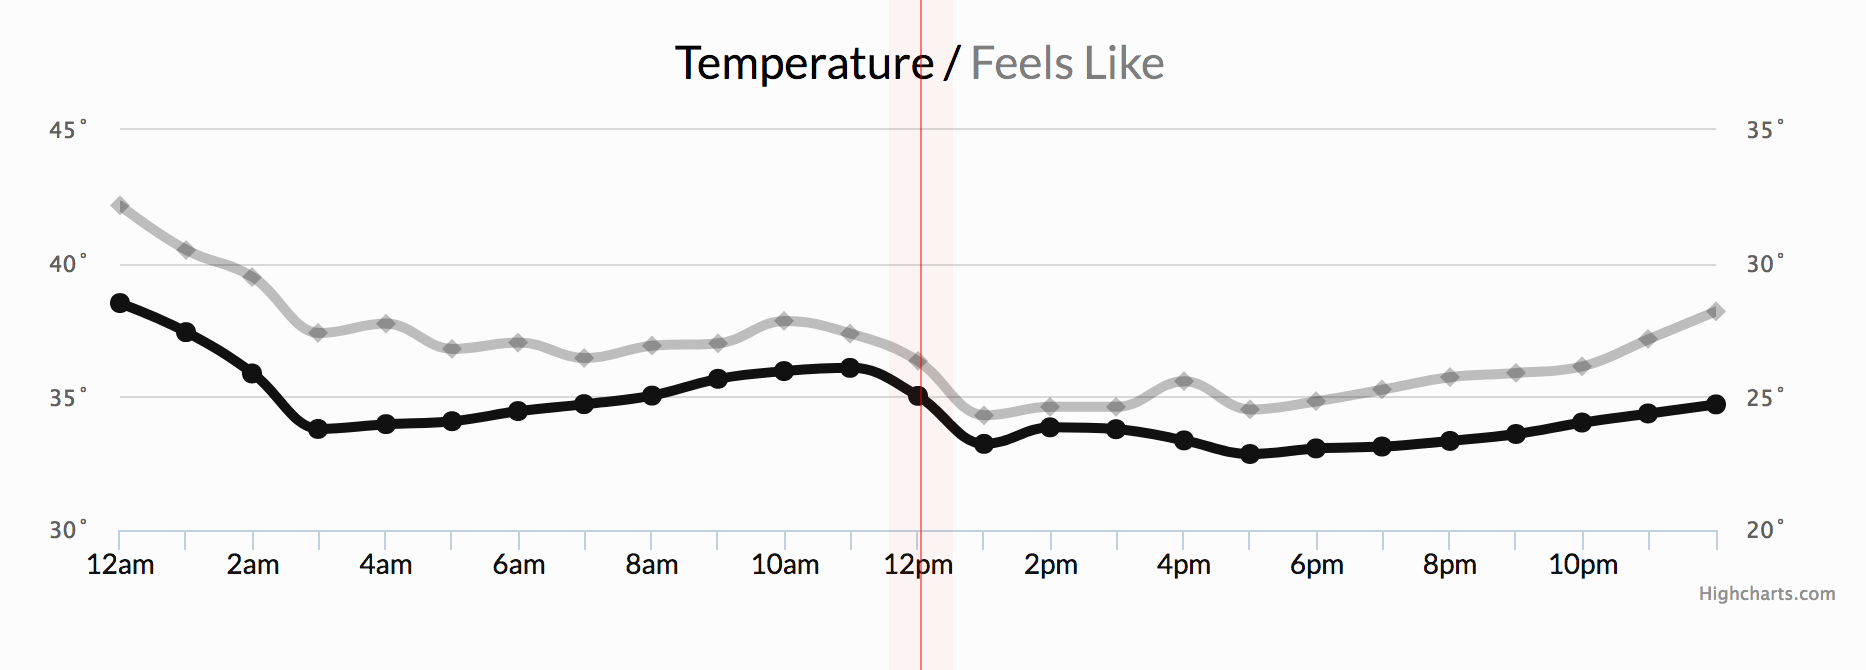
\includegraphics[width=0.7\textwidth]{figuras/dado_temporal.png}
    \caption{Exemplo de dado temporal: Condições meteorológicas}
    \label{fig:dado_temporal}
\end{figure}

\begin{figure}[h]
    \centering
    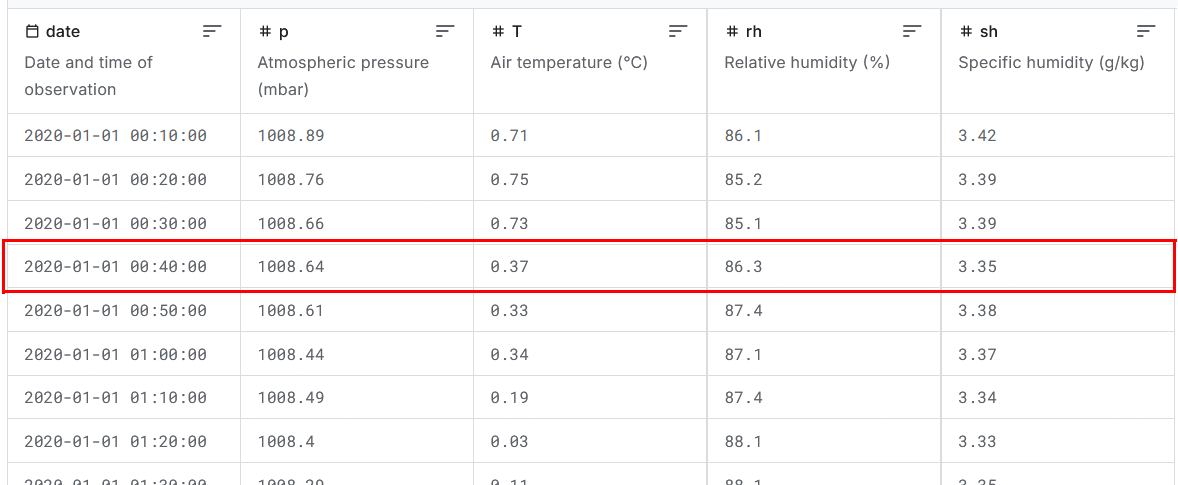
\includegraphics[width=1\textwidth]{figuras/registro_temporal.png}
    \caption{Exemplo de registro de dado temporal em um TSDB}
    \label{fig:registro_temporal}
\end{figure}

A Figura \ref{fig:dado_temporal} apresenta uma série temporal de condições meteorológicas. O elemento destacado em vermelho dentro do gráfico corresponde a um dado temporal único, um registro individual no TSDB capturado pelo sensor naquele instante.

Já a Figura \ref{fig:registro_temporal} apresenta uma tabela de um TSDB, representando a série temporal de condições meteorológicas. O elemento destacado em vermelho na tabela corresponde a um registro de um dado temporal único, com informações de data e hora, pressão atmosférica, temperatura do ar, umidade, entre outros.

Conforme explicado por \citeonline{Ozsu2011}, normalmente, uma série temporal consiste apenas em valores numéricos, sejam eles contínuos ou discretos. Consequentemente, é possível modelar fluxos de dados que contêm apenas valores numéricos como séries temporais. Isso permite usar técnicas de análise que foram desenvolvidas para séries temporais em alguns tipos de fluxo de dados. Uma característica importante é que os conjuntos de dados de séries temporais são normalmente usados em situações em que as medições, uma vez feitas, não são revisadas ou atualizadas, mas sim acumuladas, com novos dados adicionados para cada parâmetro medido em cada novo ponto no tempo \citeonline{Dunning2014}.

A importância histórica das séries temporais é notável, com exemplos que remontam ao século XIX. \citeonline{Dunning2014} mencionam o trabalho pioneiro de Matthew Fontaine Maury, que analisou registros de navios para criar cartas de ventos e correntes, demonstrando como a análise coletiva de dados de séries temporais acumulados ao longo de muitos anos em diários de bordo de muitos navios poderia revelar padrões valiosos para a navegação marítima. Esse exemplo histórico ilustra como os conjuntos de dados de séries temporais podem revelar tendências e padrões que não são aparentes em medições pontuais.

No contexto moderno, os TSDBs enfrentam novos desafios devido ao volume, velocidade e variedade dos dados gerados. Como observam \citeonline{Dunning2014}, o que antes era coletado em 10 minutos para alguns sistemas muito ativos agora é gerado a cada segundo. Essa explosão na quantidade de dados exige novas abordagens para armazenamento e acesso, tornando os bancos de dados NoSQL particularmente adequados para essa tarefa. Os autores argumentam que para consultas baseadas em tempo em escalas muito grandes, os acessos baseados em tempo podem ser implementados como varreduras grandes e contíguas que são muito eficientes se os dados forem armazenados adequadamente em um banco de dados de séries temporais.

A arquitetura dos TSDBs modernos evoluiu significativamente. \citeonline{Dunning2014} descrevem três abordagens principais para o armazenamento de séries temporais: (1) tabelas largas (\textit{wide tables}) que armazenam os dados ponto a ponto, (2) design híbrido que mistura tabelas largas com armazenamento em blobs, e (3) inserção direta de blobs a partir de um cache na memória. A abordagem de inserção direta de blobs é particularmente interessante, pois permite taxas de ingestão que podem ser até 1.000 vezes mais rápidas do que o sistema era capaz de ingerir dados sem a inserção direta de blobs.

As aplicações dos TSDBs são diversas e crescentes. \citeonline{Dunning2014} destacam casos de uso em setores como negociação de ações, telecomunicações, monitoramento de data centers e manutenção preditiva. Na área financeira, por exemplo, os autores observam que a velocidade das negociações e, portanto, a coleta de dados de negociação e a necessidade em muitos casos de latência extremamente pequena tornam o uso de bancos de dados de séries temporais de alto desempenho extremamente importante. Já no contexto da Internet das Coisas (IoT), os TSDBs ocupam uma posição central, pois ficam no coração do fluxo de dados de sensor para insight que está mudando rapidamente a maneira como percebemos e entendemos o mundo ao nosso redor.

Uma característica fundamental dos TSDBs é sua otimização para padrões específicos de consulta. Como explicam \citeonline{Dunning2014}, um banco de dados de séries temporais é uma maneira de armazenar várias séries temporais de forma que as consultas para recuperar dados de uma ou algumas séries temporais para um intervalo de tempo específico sejam particularmente eficientes. Essa eficiência é alcançada através de estratégias de armazenamento que agrupam dados temporais próximos fisicamente no armazenamento, permitindo operações de varredura sequencial eficientes.

A evolução dos TSDBs continua com o desenvolvimento de novas capacidades, como bancos de dados geo-temporais que incorporam informações de localização além do tempo. \citeonline{Dunning2014} preveem que a combinação de escala cada vez maior e mais tecnologias emergentes para coletar e analisar dados para insights valiosos está criando o desejo e a capacidade de fazer coisas novas. Essa visão aponta para um futuro onde os TSDBs desempenharão um papel ainda mais central na análise de dados em diversos domínios aplicados.

\section{Benchmarks}

A avaliação de desempenho constitui um aspecto crucial no processo de seleção de sistemas de gerenciamento de banco de dados. Conforme destacado por \citeonline{Ramakrishnan2003}, quando um banco de dados atinge dimensões que ultrapassam a capacidade do SGBD atual em fornecer desempenho satisfatório, mesmo com o melhor projeto possível, torna-se necessário considerar a migração para um novo sistema. Neste contexto, os benchmarks emergem como ferramentas essenciais para permitir comparações objetivas entre diferentes produtos disponíveis no mercado.

\citeonline{Silberschatz2020} argumenta sobre a importância de realizar testes de benchmark específicos para cada caso de uso. Como um único teste não é suficiente, utiliza-se um benchmark que simula cargas de trabalho reais, já que cada produto pode ter desempenho variado conforme a tarefa.

A complexidade inerente aos SGBDs e as diferentes abordagens adotadas pelos fornecedores tornam os benchmarks particularmente valiosos. Como observam \citeonline{Ramakrishnan2003}, um SGBD é um software complexo, e diferentes fornecedores podem direcionar seus sistemas para diferentes segmentos de mercado, colocando mais esforço em otimizar certas partes do sistema ou escolhendo diferentes projetos de sistema. Esta diversidade de enfoques e otimizações específicas dificulta a comparação direta entre sistemas, tornando os benchmarks padronizados instrumentos indispensáveis para auxiliar os usuários na seleção de um SGBD adequado às suas necessidades particulares.

No que diz respeito às características fundamentais de um bom benchmark, \citeonline{Ramakrishnan2003} enumeram três qualidades essenciais. Em primeiro lugar, a portabilidade, que se refere à capacidade do benchmark de ser executado em diferentes plataformas e sistemas. Em segundo lugar, a clareza, que garante a fácil compreensão do que está sendo efetivamente medido. Por fim, a escalabilidade, que permite a adaptação natural a instâncias maiores do problema. Além desses atributos básicos, os benchmarks ideais devem ser capazes de medir tanto o desempenho máximo, expresso em métricas como transações por segundo, quanto a relação custo-benefício, calculada em termos como dólar por transação por segundo, para cargas de trabalho típicas em um determinado domínio de aplicação. Foi precisamente para atender a essas necessidades que o Transaction Processing Council (TPC) foi criado, com a missão específica de desenvolver benchmarks padronizados para sistemas de processamento de transações e bancos de dados.

Além disso, \citeonline{Silberschatz2020} complementa que é importante calcular corretamente o desempenho médio: usar a média simples de throughputs pode induzir ao erro. O método adequado é calcular o tempo total para executar uma carga mista e, a partir disso, obter o throughput médio ou usar a média harmônica, que reflete melhor a realidade quando há diferentes tipos de transações.

A literatura especializada, conforme apresentada por \citeonline{Ramakrishnan2003}, categoriza os principais benchmarks disponíveis no mercado em três grupos principais. O primeiro grupo compreende os benchmarks de processamento de transações on-line, dentre os quais se destacam o TPC-A e TPC-B, que estabelecem as definições padrão para medidas de transações por segundo e custo por transação. Enquanto o TPC-A avalia o desempenho de toda uma rede de computadores incluindo o SGBD, o TPC-B concentra-se especificamente no sistema de gerenciamento de banco de dados. O TPC-C, por sua vez, representa uma evolução significativa em relação aos seus predecessores, modelando um ambiente complexo de armazém que rastreia itens fornecidos aos clientes através de cinco tipos diferentes de transações. Como explicam os autores, cada transação TPC-C é muito mais cara que uma transação TPC-A ou TPC-B, e o TPC-C exercita uma gama muito mais ampla de capacidades do sistema, o que levou este benchmark a substituir amplamente os anteriores como padrão para avaliação de processamento de transações.

O segundo grupo importante de benchmarks é dedicado especificamente à avaliação de desempenho em consultas. Nesta categoria, o Benchmark Wisconsin se destaca como ferramenta amplamente utilizada para medir o desempenho de consultas relacionais simples. Para cenários mais complexos, o Benchmark Set Query oferece avaliação de desempenho para um conjunto de consultas mais sofisticadas, enquanto o Benchmark AS3AP se especializa em medir o desempenho de cargas mistas que incluem transações, consultas relacionais e funções utilitárias. O TPC-D merece menção especial por constituir uma suíte abrangente de consultas SQL complexas, especialmente projetadas para representar o domínio de aplicação de suporte à decisão. Complementando esta categoria, o Benchmark do OLAP Council foi desenvolvido especificamente para avaliar consultas complexas de suporte à decisão, incluindo algumas que não podem ser expressas facilmente em SQL, sendo particularmente adequado para sistemas de processamento analítico on-line (OLAP).

O terceiro grupo identificado por \citeonline{Ramakrishnan2003} engloba os benchmarks especializados para bancos de dados de objetos. Neste domínio, os Benchmarks 001 e 007 foram concebidos especificamente para medir o desempenho de sistemas de banco de dados orientados a objetos, enquanto o Benchmark Bucky foi desenvolvido para avaliar sistemas de banco de dados objeto-relacionais, representando uma ponte entre os paradigmas relacional e orientado a objetos.

Quanto à utilização adequada desses benchmarks na prática, \citeonline{Ramakrishnan2003} oferecem diretrizes valiosas para garantir que os resultados sejam interpretados corretamente. A primeira consideração diz respeito à relevância do benchmark em si, alertando que métricas que tentam resumir o desempenho em um único número podem ser excessivamente simplistas, dado que um SGBD é um software complexo utilizado em diversas aplicações. Um bom benchmark deve, portanto, incluir uma suíte abrangente de tarefas cuidadosamente selecionadas para cobrir um domínio de aplicação específico e testar os recursos do SGBD que são críticos para aquele domínio. A segunda diretriz enfatiza a importância de analisar quão bem o benchmark reflete a carga de trabalho real do ambiente onde o SGBD será utilizado, recomendando que se dê maior peso ao desempenho nas tarefas do benchmark que mais se assemelham às operações críticas da aplicação pretendida. Finalmente, os autores sugerem a criação de benchmarks personalizados, adaptando benchmarks padrão ou substituindo suas tarefas por operações mais representativas da carga de trabalho específica do usuário, como forma de contornar possíveis otimizações específicas que os fornecedores possam ter implementado para obter bons resultados nos testes padronizados.